\documentclass[border=1pt]{standalone}

\usepackage{pgfplots}
\pgfplotsset{compat=1.18}

\begin{document}
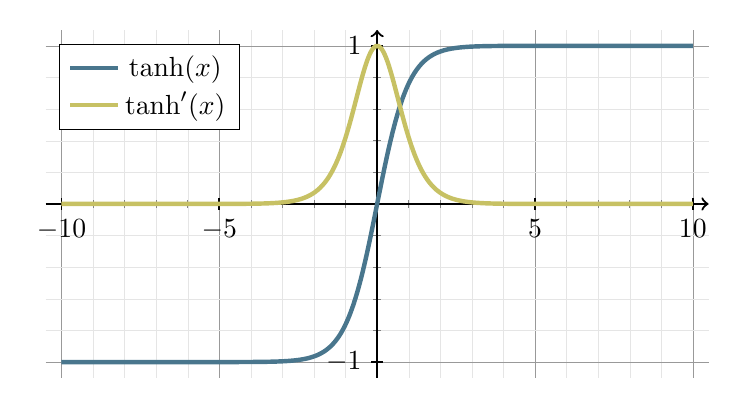
\begin{tikzpicture}[
    declare function={
        tanhp(\x)=1 - tanh(\x)*tanh(\x);
      },
    ultra thick
  ]
  \begin{axis}[
      scale=1,
      width=10cm,
      height=6cm,
      xmin=-10.5,xmax=10.5,
      ymin=-1.1,ymax=1.1,
      axis x line=center,  axis y line=center,
      minor x tick num=4,
      minor y tick num=4,
      axis line style={-to, thick},
      grid=both,
      grid style={line width=.1pt, draw=gray!20},
      major grid style={line width=.2pt,draw=gray!80},
      xtick={-10, -5,...,10},
      ytick={-1,0,..., 1},
      every major tick/.style = {
          black, semithick,
        },
      /pgf/number format/.cd, use comma,
      domain=-10:10,
      legend style={at={(0.02,0.96)},anchor=north west}
    ]
    \addplot[ultra thick, cyan!50!black, smooth, samples=250] (x,{tanh(x)});
    \addplot[ultra thick, yellow!50!gray, smooth, samples=250] (x,{tanhp(x)});
    \legend{$\tanh(x)$,$\tanh'(x)$}
  \end{axis}
\end{tikzpicture}
\end{document}
